\newgeometry{top=1.2cm, bottom=1.5cm}
\section*{Sprint Information}

\begin{itemize}[noitemsep]
    \item \textbf{Project Name:} Lab Equipment Knowledge Hub
    \item \textbf{Customer Name:} Zeth Danielsson
    \item \textbf{Sprint Number:} 1
    \item \textbf{Start Date:} September 16
    \item \textbf{End Date:} September 25
    \item \textbf{Sprint Demo Date and Time:} September 23, 15:00
    \item \textbf{Sprint Goal:} All users can log in and view created items. Elevated users can create new users and create new items.
\end{itemize}

\section*{Backlog}

\begin{figure}[h!]
\begin{adjustwidth}{-3cm}{-3cm}
\centering
    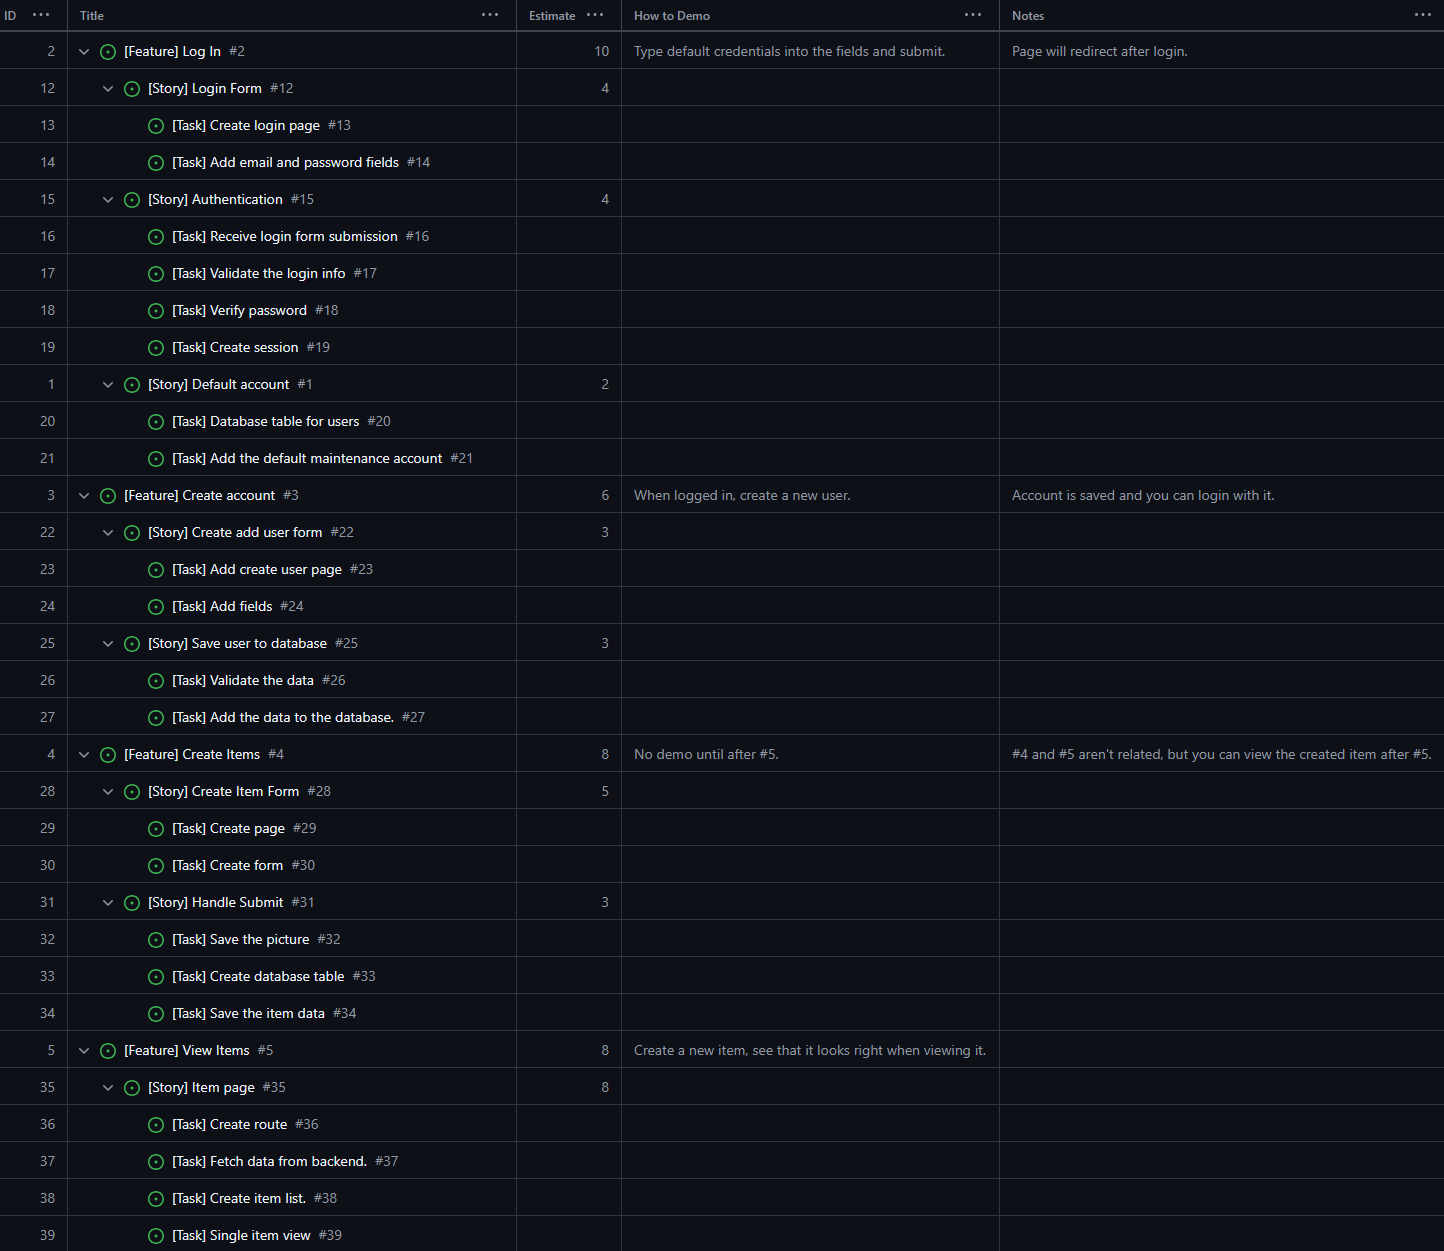
\includegraphics[width=20cm]{sprint1}
\end{adjustwidth}

    \caption*{All in all 32 hours. You can find this view as a tab in my project board. Please note that even though some estimates might seem high, some implied groundwork and scaffolding are included in the estimates. I think it is still in the same vein as "ideal hours" though.}
\end{figure}
\restoregeometry


